
\part{Structure d'un ordinateur}

\section{Éléments}

\begin{frame}
\frametitle{Structure d'un ordinateur}


Un ordinateur comporte
un \emph{processeur},
de la \emph{mémoire}, 
des \emph{dispositifs d'entrée-sortie}.

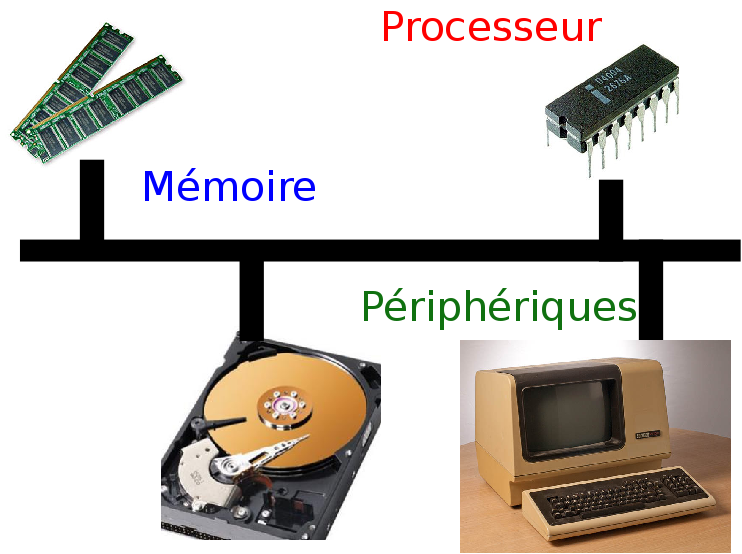
\includegraphics[width=0.8\linewidth]{figures/proc-mem-periph}

\end{frame}

\section{Interaction des éléments}
\begin{frame}
\frametitle{Rôle des éléments}
Ces éléments interagissent : 
\begin{itemize}
\item la \alert{mémoire} contient les \alert{données},
\item le \alert{processeur} exécute les \alert{instructions}
prises dans la mémoire ;
\item ces instructions 
\begin{itemize}
\item effectuent des calculs, 
\item prennent et placent des données 
en mémoire, 
\item les envoient ou les lisent sur les dispositifs d'entrée-sortie
\end{itemize}
\item les \alert{périphériques} assurent
\begin{itemize}
\item le stockage des données à long terme
\item la communication avec l'environnement
\end{itemize}
\end{itemize}

\end{frame}


\section{Le premier ordinateur}
\begin{frame}
\frametitle{SSEM : le premier ordinateur}

\alert{Small-Scale Experimental Machine}, Université de Manchester, 1948

\begin{center}
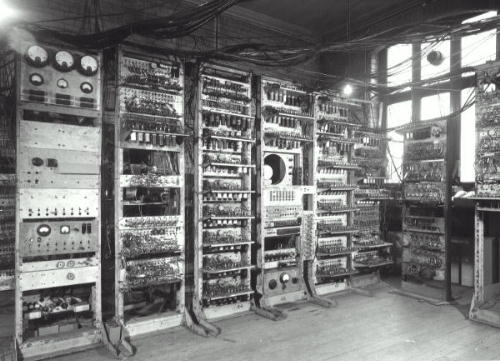
\includegraphics[width=0.6\linewidth]{images/ssem01-2.jpg}
\end{center}
Première machine à \alert{architecture Von Neumann} : \\
\alert{instructions et données} enregistrés {en mémoire}.
\end{frame}

\begin{frame}
\frametitle{SSEM, un calculateur expérimental}
\begin{itemize}
\item \alert{banc de test} pour une nouvelle technologie de mémoire :
  les tubes de Wilkins-Kilburn
\begin{tabular}{lc}
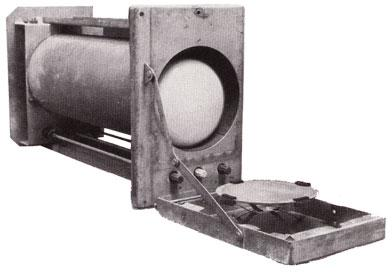
\includegraphics[width=4cm]{images/Williams-tube.jpg} &
 un tube :  32 mots de 32 bits
\end{tabular}
\item \alert{très limité}
\begin{itemize}
\item 330 diodes, 250 pentodes, 
\item un accumulateur 32 bits
\item mémoire de 32 mots
\item 7 opérations, pas d'entrées-sorties
\end{itemize}
\end{itemize}
\end{frame}



\begin{frame}
\frametitle{SSEM : démonstration concluante}

\begin{block}{Démonstration du 21 juin 1948}
\begin{itemize}
\item programme de 17 instructions,
\item 3,5 millions d'instruction en 52 minutes, soit 1,1 KIPS
\end{itemize}
\end{block}


\begin{itemize}
\item Fiabilité des tubes de Williams-Kilburn
  \begin{itemize}
  \item des heures / millions d'opérations sans erreur !
  \item employés dans le premier ordinateur d'IBM (1952)
    \\ IBM 701 : 32 tubes de Williams
    \item ensuite remplacés par les \alert{mémoires à tores de ferrite}
\item et les \alert{mémoires à semi-conducteurs} (fin années 70)
  \end{itemize}
\item \alert{Validation du concept d'ordinateur} : calculateur à programme 
  enregistré en mémoire vive 
\item Début d'une série d'ordinateurs britanniques : \\
  Mark 1, Ferranti
  Mark 1 (1951, premier ordinateur commercialisé), LEO I, II, et III (fabriqués par Lyons), etc.
\end{itemize}
\end{frame}







\section{De nos jours}

\begin{frame}
  \frametitle{De nos jours}
Processeurs beaucoup plus complexes :
plusieurs coeurs,  des lignes de caches,  des coprocesseurs etc.

\alert{Évolution du nombre de transistors par processeur}
\begin{center}
\begin{tabular}{|l|r|l|}
\hline
année &  transistors & processeur\\
\hline
1971 & 2,300 & Intel 4004, premier microprocesseur \\
1978 & 29,000 & Intel 8086, premiers PC \\
1979 & 68,000 & Motorola 68000 \\
1989 &	1,180,000 & Intel 80486 \\
1993 & 	3,100,000 & Pentium \\
1997 & 	9,500,000  & Pentium III \\
2000 & 42,000,000 & Pentium 4 \\
2012 & 1,400,000,000 & Quad-Core + GPU Core i7 \\
2012 & 5,000,000,000  & 62-Core Xeon Phi \\
\hline
\end{tabular}
\end{center}

Source : \url{http://en.wikipedia.org/wiki/Transistor_count}
\end{frame}


\part{Structure d'un processeur}

\section{Principes}

\begin{frame}
  \frametitle{Principes de base d'un processeur}

\begin{multicols}{2}
Dans un processeur il y a 
\begin{itemize}
\item des \alert{registres}  : circuits capables de mémoriser
quelques bits d'information
\item  des \alert{circuits combinatoires} (additionneur, comparateurs, ...),
\item de la \alert{logique séquentielle} pour gérer  le déroulement des différentes phases des instructions
\end{itemize}

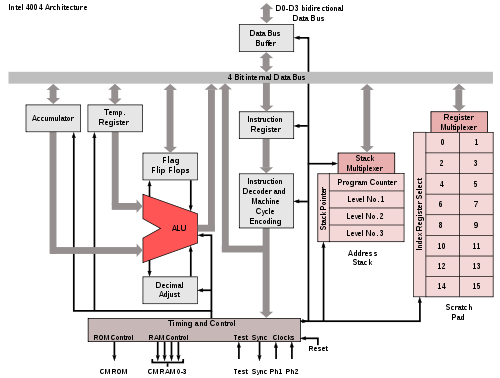
\includegraphics[width=\linewidth]{images/4004_arch.png}
\end{multicols}

\end{frame}

\section{Quelques exemples}

\begin{frame}
  \frametitle{Illustration : architecture du INTEL 4004}
  \begin{center}
  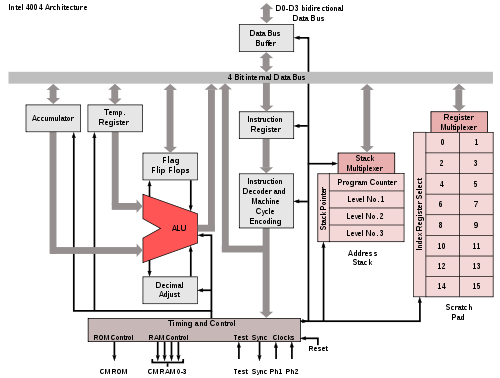
\includegraphics[width=0.8\linewidth]{images/4004_arch.png}
  \end{center}
\end{frame}

\begin{frame}
  \frametitle{Illustration : Architecture ARM, Cortex M3}
  \begin{center}
    
  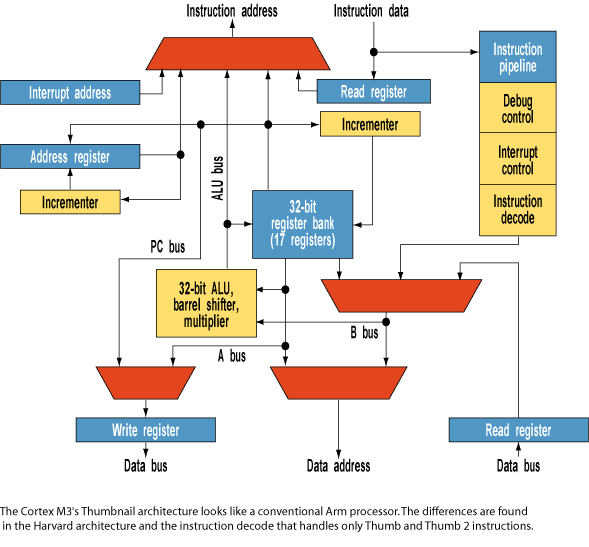
\includegraphics[width=0.6\linewidth]{images/arm-arch.png}
  \end{center}
\end{frame}

\section{Modèle du programmeur}

\begin{frame}
\frametitle{le ``Modèle du programmeur''}
  Le programmeur n'a pas à connaître tous ces détails, seulement 
\begin{itemize}
\item le jeu d'instructions qu'il peut employer

\begin{itemize}
\item les \alert{différents types d'instruction}
\item leur effet sur les registres accessibles
\end{itemize}
\item les registres auquel il a accès
  \begin{itemize}
  \item le \alert{compteur de programme} (adresse de la prochaine instruction)
  \item les \alert{registres} de travail,
\item les \alert{indicateurs de condition}
\item ...
  \end{itemize}
\end{itemize}
\end{frame}


